\documentclass[10pt,a4paper,]{article}

%% %%%%%%%%%%%%%%%%%%%%%%%%%%%%%%%%%%%%%%%%%%%%%%%%%%%%%%%%%%%%%%%%%%%%%%%%%%%%%%%%%%%%%%
%%
%%   BScBI_CompGenomics_template.tex
%%
%%   A LaTeX template for MarkDown reports to submit as BScBI-CG practical exercises.
%%
%% %%%%%%%%%%%%%%%%%%%%%%%%%%%%%%%%%%%%%%%%%%%%%%%%%%%%%%%%%%%%%%%%%%%%%%%%%%%%%%%%%%%%%%
%%
%%                 CopyLeft 2024 (CC:BY-NC-SA) --- Josep F Abril
%%
%%   This file should be considered under the Creative Commons BY-NC-SA License
%%   (Attribution-Noncommercial-ShareAlike). The material is provided "AS IS", 
%%   mainly for teaching purposes, and is distributed in the hope that it will
%%   be useful, but WITHOUT ANY WARRANTY; without even the implied warranty
%%   of MERCHANTABILITY or FITNESS FOR A PARTICULAR PURPOSE.
%%
%% %%%%%%%%%%%%%%%%%%%%%%%%%%%%%%%%%%%%%%%%%%%%%%%%%%%%%%%%%%%%%%%%%%%%%%%%%%%%%%%%%%%%%%

\usepackage[pdftex]{graphicx}
\usepackage{xcolor} %%% FIX %%%
\usepackage{fancyvrb}
\usepackage{comment}
\usepackage{fancyhdr} % Do not use \usepackage{fancybox} -> TOCs disappear
\usepackage{multirow}
\usepackage[nottoc,notlof,notlot,numbib]{tocbibind}

\usepackage{lmodern}
\usepackage{amssymb,amsmath}
\usepackage{ifxetex,ifluatex}
\usepackage{fixltx2e} % provides \textsubscript
\ifnum 0\ifxetex 1\fi\ifluatex 1\fi=0 % if pdftex
  \usepackage[T1]{fontenc}
  \usepackage[utf8]{inputenc}
\else % if luatex or xelatex
  \ifxetex
    \usepackage{mathspec}
    \usepackage{xltxtra,xunicode}
  \else
    \usepackage{fontspec}
  \fi
  \defaultfontfeatures{Mapping=tex-text,Scale=MatchLowercase}
  \newcommand{\euro}{€}
\fi
% use upquote if available, for straight quotes in verbatim environments
\IfFileExists{upquote.sty}{\usepackage{upquote}}{}
% use microtype if available
\IfFileExists{microtype.sty}{%
\usepackage{microtype}
\UseMicrotypeSet[protrusion]{basicmath} % disable protrusion for tt fonts
}{}
\usepackage[margin=1.5cm]{geometry}
\usepackage{natbib}
\bibliographystyle{plainnat}
\usepackage{color}
\usepackage{fancyvrb}
\newcommand{\VerbBar}{|}
\newcommand{\VERB}{\Verb[commandchars=\\\{\}]}
\DefineVerbatimEnvironment{Highlighting}{Verbatim}{commandchars=\\\{\}}
% Add ',fontsize=\small' for more characters per line
\newenvironment{Shaded}{}{}
\newcommand{\AlertTok}[1]{\textcolor[rgb]{1.00,0.00,0.00}{\textbf{#1}}}
\newcommand{\AnnotationTok}[1]{\textcolor[rgb]{0.38,0.63,0.69}{\textbf{\textit{#1}}}}
\newcommand{\AttributeTok}[1]{\textcolor[rgb]{0.49,0.56,0.16}{#1}}
\newcommand{\BaseNTok}[1]{\textcolor[rgb]{0.25,0.63,0.44}{#1}}
\newcommand{\BuiltInTok}[1]{#1}
\newcommand{\CharTok}[1]{\textcolor[rgb]{0.25,0.44,0.63}{#1}}
\newcommand{\CommentTok}[1]{\textcolor[rgb]{0.38,0.63,0.69}{\textit{#1}}}
\newcommand{\CommentVarTok}[1]{\textcolor[rgb]{0.38,0.63,0.69}{\textbf{\textit{#1}}}}
\newcommand{\ConstantTok}[1]{\textcolor[rgb]{0.53,0.00,0.00}{#1}}
\newcommand{\ControlFlowTok}[1]{\textcolor[rgb]{0.00,0.44,0.13}{\textbf{#1}}}
\newcommand{\DataTypeTok}[1]{\textcolor[rgb]{0.56,0.13,0.00}{#1}}
\newcommand{\DecValTok}[1]{\textcolor[rgb]{0.25,0.63,0.44}{#1}}
\newcommand{\DocumentationTok}[1]{\textcolor[rgb]{0.73,0.13,0.13}{\textit{#1}}}
\newcommand{\ErrorTok}[1]{\textcolor[rgb]{1.00,0.00,0.00}{\textbf{#1}}}
\newcommand{\ExtensionTok}[1]{#1}
\newcommand{\FloatTok}[1]{\textcolor[rgb]{0.25,0.63,0.44}{#1}}
\newcommand{\FunctionTok}[1]{\textcolor[rgb]{0.02,0.16,0.49}{#1}}
\newcommand{\ImportTok}[1]{#1}
\newcommand{\InformationTok}[1]{\textcolor[rgb]{0.38,0.63,0.69}{\textbf{\textit{#1}}}}
\newcommand{\KeywordTok}[1]{\textcolor[rgb]{0.00,0.44,0.13}{\textbf{#1}}}
\newcommand{\NormalTok}[1]{#1}
\newcommand{\OperatorTok}[1]{\textcolor[rgb]{0.40,0.40,0.40}{#1}}
\newcommand{\OtherTok}[1]{\textcolor[rgb]{0.00,0.44,0.13}{#1}}
\newcommand{\PreprocessorTok}[1]{\textcolor[rgb]{0.74,0.48,0.00}{#1}}
\newcommand{\RegionMarkerTok}[1]{#1}
\newcommand{\SpecialCharTok}[1]{\textcolor[rgb]{0.25,0.44,0.63}{#1}}
\newcommand{\SpecialStringTok}[1]{\textcolor[rgb]{0.73,0.40,0.53}{#1}}
\newcommand{\StringTok}[1]{\textcolor[rgb]{0.25,0.44,0.63}{#1}}
\newcommand{\VariableTok}[1]{\textcolor[rgb]{0.10,0.09,0.49}{#1}}
\newcommand{\VerbatimStringTok}[1]{\textcolor[rgb]{0.25,0.44,0.63}{#1}}
\newcommand{\WarningTok}[1]{\textcolor[rgb]{0.38,0.63,0.69}{\textbf{\textit{#1}}}}
% .if(graphics).
% \usepackage{graphicx}
% \makeatletter
% \def\maxwidth{\ifdim\Gin@nat@width>\linewidth\linewidth\else\Gin@nat@width\fi}
% \def\maxheight{\ifdim\Gin@nat@height>\textheight\textheight\else\Gin@nat@height\fi}
% \makeatother
% % Scale images if necessary, so that they will not overflow the page
% % margins by default, and it is still possible to overwrite the defaults
% % using explicit options in \includegraphics[width, height, ...]{}
% \setkeys{Gin}{width=\maxwidth,height=\maxheight,keepaspectratio}
% .endif.
\ifxetex
  \usepackage[setpagesize=false, % page size defined by xetex
              unicode=false, % unicode breaks when used with xetex
              xetex]{hyperref}
\else
  \usepackage[unicode=true]{hyperref}
\fi
\hypersetup{breaklinks=true,
            bookmarks=true,
            pdfauthor={Bruno Alvarez @ BScBI Computational Genomics},
            pdftitle={BScBI-CG Exercise 00},
            colorlinks=true,
            citecolor=green,
            urlcolor=blue,
            linkcolor=red,
            pdfborder={0 0 0}}
\urlstyle{same}  % don't use monospace font for urls
\setlength{\parindent}{0pt}
\setlength{\parskip}{6pt plus 2pt minus 1pt}
\setlength{\emergencystretch}{3em}  % prevent overfull lines
\setcounter{secnumdepth}{5}

%%% Sequence units
\usepackage{siunitx}
\DeclareSIUnit\molar{\mole\per\cubic\deci\metre}
\DeclareSIUnit\Molar{\textsc{m}}
\DeclareSIUnit\bp{bp}
\DeclareSIUnit\kbp{\kilo\bp}
\DeclareSIUnit\Mbp{\mega\bp}
\DeclareSIUnit\Gbp{\giga\bp}
\DeclareSIUnit\X{{\footnotesize\textsf{X}}}

%%% Compute current time using 24Hr. notation
{\count1=\time \divide\count1 by 60 \multiply\count1 by 60 %
 \count2=\time \advance\count2 by -\count1 %
 \divide\count1 by 60 %
 \xdef\currenttime{\the\count1:\ifnum\count2<10 0\fi\the\count2}}
\newcommand{\tstamp}{\textbf{\today\ /\ \currenttime}}

%%% Header/Footer Stuff
\def\thylab{\textbf{BSc BI --- Computational Genomics}}
\def\thylogo{\phantom{x}\raisebox{-2mm}{
\includegraphics[height=6.5mm, width=6.5mm]{{docs/ESCI_logo}.png}}} %%% FIX %%%
%
\fancyhead{} % clear all fields
\fancyfoot{} % clear all fields
\fancyhead[RO,LE]{\thepage}
%\fancyhead[LO,RE]{\shorttit\quad\rightmark}
\fancyhead[LO]{\small{}BScBI-CG Exercise 00 Report}
\fancyhead[RE]{\small{}\rightmark}
\fancyfoot[LO,LE]{\small\textbf{\thylab}}
\fancyfoot[CO,CE]{\small\textsl{Alvarez, B}}
\fancyfoot[RO,RE]{\small\textbf{\today}\thylogo}
\renewcommand{\headrulewidth}{1pt}
\renewcommand{\footrulewidth}{1.5pt}

%.if(title).
%\title{.title..if(subtitle).\\\vspace{0.5em}{\large .subtitle.}.endif.}
%.endif.
\author{true}
\date{}

%% smaller font for code blocs...
\makeatletter
\newcommand{\verbatimfont}[1]{\renewcommand{\verbatim@font}{\ttfamily#1}}
\makeatother
\verbatimfont{\footnotesize}%

%% embedding external files
\newcommand{\loadfile}[3]{% BOXLABEL (escape "_") // ./relativepathtofile/FILENAME // REFLABEL
  \phantomsection\label{#3}\VerbatimInput[frame=single,framesep=5mm,fontsize=\footnotesize,label=\fbox{#1}]{#2}
}%

\providecommand{\tightlist}{%
  \setlength{\itemsep}{0pt}\setlength{\parskip}{0pt}}

\def\CGVC{\href{https://aula.esci.upf.edu/course/view.php?id=8516}{Computational Genomics Virtual Campus at ESCI}}

\begin{document}

%
\thispagestyle{empty}
%
\begin{titlepage}
\begin{center}
%
\ \vfill
%
\textbf{\Huge \textsc{BScBI-CG} \vskip 1.25ex \textsc{Practicals}
\vskip 1.25ex \textsc{Report}}\\[6ex]
%
\textbf{\Large%
\href{mailto:bruno.alvarez@alum.esci.upf.edu?subject=[BScBI-CG Exercise
00]}{Bruno Alvarez}%
}\\%
\vskip 8ex
\textbf{\huge Exercise 00}
\vskip 8ex
\textbf{\large --- \today ---}
%
\end{center}
\vfill
%
%\begin{raggedright}
\hfill\begin{tabular}{r@{\hspace{1em}}l}

\includegraphics[height=2cm, width=4cm]{{docs/ESCI_logo}.png}
& %
\shortstack{%
\textbf{\textsc{\large Computational Genomics 2024--25}}\\[1ex]
\textsc{BSc in Bioinformatics}\\[1.25ex]
% {\large \href{http://www.upf.edu/en/}{UPF} -- \href{http://www.fib.upc.edu/en/bioinformatica.html}{UPC} -- \href{http://www.ub.edu/web/ub/en/estudis/oferta_formativa/graus/fitxa/B/G1091/index.html?}{UB}}%
{\large \href{https://www.esci.upf.edu/en/bachelors-degree-in-bioinformatics/bachelors-degree-bioinformatics}{UPF/ESCI} -- \href{https://www.upc.edu/en/bachelors/bioinformatics-interuniversity-upf-upc-ub-uab-degree-barcelona-fib}{UPC} -- \href{https://web.ub.edu/en/web/estudis/w/bachelordegree-g1134}{UB} -- \href{https://www.uab.cat/web/estudiar/ehea-degrees/general-information/bioinformatics-uab/upf/ub/upc-1216708259085.html?param1=1345746721560}{UAB}}%
}%shortstack
\\[2ex]
\end{tabular}
%\end{raggedright}
%
\end{titlepage}
%
%\maketitle
\newpage
%thytitle

{
%\hypersetup{linkcolor=black}
\pagenumbering{roman}
\setcounter{page}{1}
\setcounter{tocdepth}{3}
\tableofcontents
%
\vfill
%\newpage
}
\listoftables
\vfill
\listoffigures
\vfill
%
\newpage

\pagenumbering{arabic}
\setcounter{page}{1}
\pagestyle{fancy}

\begin{comment} 
The \texttt{comment} \LaTeX\ environment allow us to
include any piece of text, code, etc, but it wil not be included into
the final PDF report when compiling the \texttt{MarkDown} file. You
can open/close one of such environments at any time if you need them.
\end{comment}

\hypertarget{introduction}{%
\section{Introduction}\label{introduction}}

We are going to reuse a set of existing \texttt{MarkDown} report
templates to define the protocols to be run on each practical session.
This first document will allow us to describe the different sections it
contains, highlighting the major blocks its made of. We will also use it
to provide applied examples of the \texttt{MarkDown} and \LaTeX~syntax;
for both we will introduce new features on each new practical session.
You can read the
\href{http://daringfireball.net/projects/markdown/syntax\#link}{\texttt{MarkDown}
syntax guide}, as well as from the manual pages (just type
\texttt{man\ pandoc} and/or \texttt{man\ pandoc\_markdown} if you have
installed this software tool).

\hypertarget{objectives}{%
\subsection{Objectives}\label{objectives}}

\begin{itemize}
\tightlist
\item
  We will practice how to report the commands and the results required
  to solve the practical exercises, using a text file, this report of
  course, and the \texttt{MarkDown} syntax. Some enhancements using
  \LaTeX\\
  will be also illustrated.
\item
  The main goal is to understand the structure and logic of the report
  document, what can be found on each section, how code blocks are
  defined, and how to process it for submission to the
  \href{https://aula.esci.upf.edu/course/view.php?id=8516}{Computational Genomics Virtual Campus at ESCI}.
\item
  This exercise will be useful to check that all required packages and
  libraries are working properly in order to generate the practical
  reports for the continued assessment of the subject.
\item
  At the same time, if those commands can run on our computers, we will
  have some commands already installed and available for the forthcoming
  practical sessions.
\end{itemize}

\hypertarget{prerequisites}{%
\subsection{Prerequisites}\label{prerequisites}}

\hypertarget{installing-required-software}{%
\subsubsection{Installing required
software}\label{installing-required-software}}

For this practical we must ensure that at least \texttt{pandoc} and
\texttt{pdflatex} commands are running smoothly over our report files.
You probably may need to install the following packages before working
on anything else.

\hypertarget{linux-users}{%
\paragraph{\texorpdfstring{\textbf{Linux}
users:}{Linux users:}}\label{linux-users}}

You must submit an exercise report for each practical as two single
files, a \texttt{MarkDown} text file and a \texttt{PDF} compiled from
that \texttt{MarkDown} file. In order to run such procedure, we must
ensure that we have the software tools and the corresponding
dependencies. This has to be done for the first exercise only, as you
will have those tools already available for future compilations of the
other exercises. The command below will install those tools:

\begin{Shaded}
\begin{Highlighting}[]
\FunctionTok{sudo}\NormalTok{ apt{-}get install pandoc }\KeywordTok{\textbackslash{}}
                     \ExtensionTok{texlive{-}latex{-}recommended} \KeywordTok{\textbackslash{}}
                     \ExtensionTok{texlive{-}latex{-}extra} \KeywordTok{\textbackslash{}}
                     \ExtensionTok{texlive{-}fonts{-}recommended}

\CommentTok{\# getting the latest version from repository}
\CommentTok{\#     https://github.com/jgm/pandoc/releases/latest}
\CommentTok{\# for a Debian{-}based linux distribution you can run those two commands:}
\FunctionTok{wget}\NormalTok{ https://github.com/jgm/pandoc/releases/download/3.1.8/pandoc{-}3.4{-}1{-}amd64.deb}
\FunctionTok{sudo}\NormalTok{ dpkg {-}i pandoc{-}3.4{-}1{-}amd64.deb}
\end{Highlighting}
\end{Shaded}

When using \texttt{pandoc} version greater than \texttt{2.x} we will be
able to apply further macros and tags on our report file (like embed
\texttt{LaTeX} blocks). In case you want to play with \LaTeX, I will
recommend you to install the complete set with this command (it takes
some time to download them though, as you may get the packages and many
dependencies):

\begin{Shaded}
\begin{Highlighting}[]
\FunctionTok{sudo}\NormalTok{ apt{-}get install texlive{-}full }\KeywordTok{\textbackslash{}}
                     \ExtensionTok{texlive{-}fonts{-}recommended} \KeywordTok{\textbackslash{}}
                     \ExtensionTok{texlive{-}fonts{-}extra}
\end{Highlighting}
\end{Shaded}

You can also install optional packages, such a text editor with
programming facilities and extensions, like \texttt{emacs} or
\texttt{geany} (you can also use \texttt{sublime}, \texttt{atom},
\texttt{gedit}, \ldots):

\begin{Shaded}
\begin{Highlighting}[]
\FunctionTok{sudo}\NormalTok{ apt{-}get install emacs geany vim vim{-}gtk}
\end{Highlighting}
\end{Shaded}

Another example of downloading source code and compiling it (\textbf{NOT
NEEDED if you are using CONDA ENVIRONMENT}).

\begin{Shaded}
\begin{Highlighting}[]
\FunctionTok{git}\NormalTok{ clone https://github.com/kimrutherford/EMBOSS.git}
\BuiltInTok{cd}\NormalTok{ EMBOSS}
\ExtensionTok{./configure}\NormalTok{ {-}{-}prefix=/usr/local/install/EMBOSS}
\FunctionTok{make}
\FunctionTok{make}\NormalTok{ check}
\FunctionTok{make}\NormalTok{ install}
\end{Highlighting}
\end{Shaded}

Further instructions will be given on the templates in case a practical
requires that you install further software\ldots{}

\hypertarget{macos-users}{%
\paragraph{\texorpdfstring{\textbf{MacOS}
users:}{MacOS users:}}\label{macos-users}}

MacOS users can try to install ports for the software tools from
\texttt{homebrew} or \texttt{conda} repositories. Here we have a brief
summary of such commands. \texttt{Homebrew} is a package manager for
\textbf{MacOS}; it also has a port for \textbf{Linux}, known as
\texttt{Linuxbrew}. To install this package manager, just copy the
following command and paste it to a Terminal window:

\begin{Shaded}
\begin{Highlighting}[]
\CommentTok{\# setting up brew tool and its repositories}
\ExtensionTok{/bin/bash}\NormalTok{ {-}c }\StringTok{"}\VariableTok{$(}\ExtensionTok{curl}\NormalTok{ {-}fsSL https://raw.githubusercontent.com/Homebrew/install/master/install.sh}\VariableTok{)}\StringTok{"}
\CommentTok{\# OLD ruby installer:}
\CommentTok{\#\# /usr/bin/ruby {-}e "$(curl {-}fsSL https://raw.githubusercontent.com/Homebrew/install/master/install)"}
\end{Highlighting}
\end{Shaded}

A list of all the available packages (known as \emph{formulae}) is found
at \href{https://formulae.brew.sh}{formulae.brew.sh}. Examples of
\texttt{brew} command to install the \texttt{EMBOSS} or the
\texttt{pandoc} are shown here:

\begin{Shaded}
\begin{Highlighting}[]
\CommentTok{\# Getting EMBOSS installed with brew}
\ExtensionTok{brew}\NormalTok{ search emboss}
\CommentTok{\# homebrew/science/emboss  \#\textless{}{-}{-} check the output of the previous command to use in your system}
\ExtensionTok{brew}\NormalTok{ install homebrew/science/emboss}

\CommentTok{\# Getting pandoc installed with brew}
\ExtensionTok{brew}\NormalTok{ install pandoc}
\CommentTok{\# this is optional}
\ExtensionTok{brew}\NormalTok{ install pandoc{-}citeproc}
\CommentTok{\# you need this to typeset PDFs with LaTeX}
\ExtensionTok{brew}\NormalTok{ install librsvg python homebrew/cask/basictex}

\CommentTok{\# You can also download the pandoc MacOS instaler from the following URL:}
\CommentTok{\# https://github.com/jgm/pandoc/releases/download/3.4/pandoc{-}3.4{-}x86\_64{-}macOS.pkg}
\end{Highlighting}
\end{Shaded}

\hypertarget{using-condamamba-environments}{%
\paragraph{\texorpdfstring{Using \texttt{conda/mamba}
environments:}{Using conda/mamba environments:}}\label{using-condamamba-environments}}

Yet another way to install the software required to complete the
exercises is to use \texttt{conda} environments. You can install
\texttt{conda} following the instructions from
\href{https://conda.io/projects/conda/en/latest/user-guide/install/index.html}{this
link}; you can also use \texttt{mamba} instead, which is a compact and
faster implementation of \texttt{conda}, from the instructions at
\href{https://github.com/conda-forge/miniforge\#install}{this link}.
Once you have one of those environment managers installed, you can
follow the commands in the next code block to create the
\texttt{BScBI-CG2425\_exercises} environment and activate it.

\begin{Shaded}
\begin{Highlighting}[]
\CommentTok{\#}
\CommentTok{\# If you have conda instead of mamba already installed on your system}
\CommentTok{\# you can just replace \textquotesingle{}mamba\textquotesingle{} by \textquotesingle{}conda\textquotesingle{} on the commands below:}
\CommentTok{\#}
\ExtensionTok{mamba}\NormalTok{ env create {-}{-}file environment.yml}

\CommentTok{\# Now you can run the tools installed on that environment by activating it:}
\ExtensionTok{mamba}\NormalTok{ activate BScBI{-}CG2425\_exercises}

\CommentTok{\# Remember that each time you deactivate a conda environment}
\CommentTok{\# all shell variables defined inside will be lost}
\CommentTok{\# (unless they were exported before activating the conda environment).}
\CommentTok{\# Anyway, you can reload project vars with:}
\BuiltInTok{source}\NormalTok{ projectvars.sh}

\CommentTok{\# To return to the initial terminal state, you must deactivate the environment:}
\ExtensionTok{mamba}\NormalTok{ deactivate}
\end{Highlighting}
\end{Shaded}

You can review the contents of the environment YAML file at the
Appendices (see section \ref{prg:environmentYML} on page
\pageref{prg:environmentYML}),

\hypertarget{using-docker-containers}{%
\paragraph{\texorpdfstring{Using \texttt{docker}
containers:}{Using docker containers:}}\label{using-docker-containers}}

If you have a MacOS, a MS-Windows OS, or you cannot deal with the
software install commands from the previous section, you can even use
the container we provide for the course, which has all those tools
already packed and ready to be used.

\begin{Shaded}
\begin{Highlighting}[]
\CommentTok{\# You must install docker server to run containers in your system.}
\CommentTok{\# Follow the instructions from the URLs below}
\CommentTok{\#    https://docs.docker.com/}
\CommentTok{\#          https://docs.docker.com/install/linux/docker{-}ce/debian/}
\CommentTok{\#          https://docs.docker.com/docker{-}for{-}mac/install/}
\CommentTok{\#          https://docs.docker.com/docker{-}for{-}windows/install/}

\CommentTok{\# Download the tarball from the course materials (take care, it\textquotesingle{}s a 3.5GB file)}
\FunctionTok{wget}\NormalTok{ https://compgen.bio.ub.edu/\textasciitilde{}jabril/teaching/BScBI{-}CG2425/MScGGBIA\_docker.tar.gz}

\CommentTok{\# Then, get the tarball unzipped on your machine:}
\FunctionTok{gunzip}\NormalTok{ {-}vc }\StringTok{\textquotesingle{}/mounted\_device\_path/MScGGBIA\_docker.tar.gz\textquotesingle{}} \OperatorTok{\textgreater{}}\NormalTok{ \textasciitilde{}/MScGGBIA\_docker.tar}

\CommentTok{\#  Upload the container to your docker server:}
\ExtensionTok{docker}\NormalTok{ load {-}i \textasciitilde{}/MScGGBIA\_docker.tar}

\CommentTok{\# Change directory on the current terminal/shell to the exercise folder.}

\CommentTok{\# Run this docker with:}
\ExtensionTok{docker}\NormalTok{ run {-}{-}rm {-}ti {-}e WD=}\StringTok{"}\VariableTok{$PWD}\StringTok{"}\NormalTok{ {-}v /home:/home   mscggbia    \# on a Linux   machine}
\ExtensionTok{docker}\NormalTok{ run {-}{-}rm {-}ti {-}e WD=}\StringTok{"}\VariableTok{$PWD}\StringTok{"}\NormalTok{ {-}v /Users:/Users mscggbia    \# on a Mac     machine}
\ExtensionTok{docker}\NormalTok{ run {-}{-}rm {-}ti {-}e WD=}\StringTok{"}\VariableTok{$pwd}\StringTok{"}\NormalTok{ {-}v c:/Users:/Users mscggbia  \# on a Windows machine }

\CommentTok{\# Now you will be inside the container on the root folder,}
\CommentTok{\# so you have to change to the working directory:}
\BuiltInTok{cd} \VariableTok{$WD}
\CommentTok{\# Then you are ready to play with commands at the exercise folder.}
\BuiltInTok{source}\NormalTok{ projectvars.sh}
\ExtensionTok{runpandoc}
\end{Highlighting}
\end{Shaded}

\hypertarget{initializing-the-main-report-files}{%
\subsubsection{Initializing the main report
files}\label{initializing-the-main-report-files}}

In a \texttt{bash} command-line terminal, create a folder for all the
practicals on this subject and change working dir to that folder:

\begin{Shaded}
\begin{Highlighting}[]
\FunctionTok{mkdir}\NormalTok{ practicals}
\BuiltInTok{cd}\NormalTok{ practicals}
\end{Highlighting}
\end{Shaded}

Then, we need to download the exercise tarball (the \texttt{*.tgz} file)
from the
\href{https://aula.esci.upf.edu/course/view.php?id=8516}{Computational Genomics Virtual Campus at ESCI}~into
that folder, unpack such file, modify the files accordingly to the user
within the exercise folder, and set it as the current working directory
for the rest of the practical session\ldots{}

\begin{Shaded}
\begin{Highlighting}[]
\CommentTok{\# Uncompress and unpack the exercise files from tarball}
\CommentTok{\#}
\CommentTok{\# }\AlertTok{NOTE}\CommentTok{: If you are reading this, you probably have already done this step.}
\CommentTok{\#}
\FunctionTok{tar}\NormalTok{ {-}zxvf BScBI\_CG2425\_exercise\_00.tgz}

\CommentTok{\# Move into the new extracted folder}
\BuiltInTok{cd}\NormalTok{ exercise\_00}

\CommentTok{\# Rename the MarkDown README\_*.md file by replacing NAME and SURNAME strings}
\CommentTok{\# with your "NAME" and "SURNAME" with the following command}
\FunctionTok{mv}\NormalTok{ {-}v README\_BScBICG2425\_exercise00\_SURNAME\_NAME.md }\KeywordTok{\textbackslash{}}
      \ExtensionTok{README\_BScBICG2425\_exercise00\_YourSurname\_YourName.md}

\CommentTok{\# Open exercise files using your text editor of choice}
\CommentTok{\# (for instance vim, emacs, gedit, sublime, atom, ...);}
\ExtensionTok{emacs}\NormalTok{  projectvars.sh }\KeywordTok{\textbackslash{}}
       \ExtensionTok{README\_BScBICG2425\_exercise00\_YourSurname\_YourName.md}

\CommentTok{\# Fix "NAME" and "SURNAME" placeholders on those files}
\CommentTok{\# and save the changes before continuing.}

\CommentTok{\# Load the bash definitions from projectvars.sh}
\BuiltInTok{source}\NormalTok{ projectvars.sh}
\CommentTok{\# for instance the variable WDR was set to the absolute path}
\CommentTok{\# to current exercise working directory}
\BuiltInTok{echo} \VariableTok{$WDR}

\CommentTok{\# Now you are ready to start the practical by looking at}
\CommentTok{\# the MarkDown file for further instructions to run}
\CommentTok{\# the corresponding code blocks.}

\CommentTok{\# Each time you include your answers/code/results}
\CommentTok{\# on the README file, you can compile it into PDF.}
\CommentTok{\# So that, let\textquotesingle{}s tests if we can compile the modified MarkDown document.}
\CommentTok{\# You probably must install some dependencies yet...}
\ExtensionTok{runpandoc}
\end{Highlighting}
\end{Shaded}

Again, remember to submit both files, the MD and the PDF, to the
\href{https://aula.esci.upf.edu/course/view.php?id=8516}{Computational Genomics Virtual Campus at ESCI},
once errors/warnings have been fixed, all the requested task have been
completed, and you have discussed your results on the corresponding
sections.

If you have succeeded on the software installation step, then you can
start with the analyses provided on the next section\ldots{} May the
shell be with you\ldots{}

\newpage

\hypertarget{genome-properties-comparison}{%
\section{Genome properties
Comparison}\label{genome-properties-comparison}}

As an example of analysis we can record in a \texttt{MarkDown} report
file, we are going to plot the distribution of lengths for a set of
eukaryotic organisms.

\hypertarget{datasets}{%
\subsection{Datasets}\label{datasets}}

We already have a file in tabular format in the \texttt{stats} folder,
where we have saved some whole-genome properties of several eukaryotic
species. The initial \texttt{genomes.csv} file was downloaded from the
\href{https://www.ncbi.nlm.nih.gov/genome/browse\#!/overview/}{Genome
Information by Organism online resource} at
\href{https://www.ncbi.nlm.nih.gov/genome/}{NCBI-Genomes database
division}. The file has info about species, their taxonomic group, the
genome size in mega-basepairs (Mbp), number of completed chromosomes and
organelles, as well as the number of available assemblies at NCBI, for a
total of 47,345 species.

\hypertarget{basic-data-checks-from-command-line}{%
\subsection{Basic data checks from
command-line}\label{basic-data-checks-from-command-line}}

We can take a look to the \texttt{genomes.csv} file contents with some
basic \textbf{Unix} comands. We will filter out some fields and records,
then we will upload the processed table into an R shell and we will
transform the data into few summary plots.

\begin{Shaded}
\begin{Highlighting}[]
\CommentTok{\#\# listing directory contents}
\FunctionTok{ls}\NormalTok{ {-}alFhrt stats/}
\CommentTok{\# drwxr{-}xr{-}x 2 jabril users 4.0K Sep 28 14:21 ./}
\CommentTok{\# drwxr{-}xr{-}x 6 jabril users 4.0K Sep 28 14:13 ../}
\CommentTok{\# {-}rw{-}r{-}{-}r{-}{-} 1 jabril users 5,9M Sep 28 14:15 genomes.csv}

\CommentTok{\#\# counting number of lines, words and chars of a file}
\FunctionTok{wc}\NormalTok{ stats/genomes.csv }
\CommentTok{\#  72068  245486 6143707 stats/genomes.csv}
\CommentTok{\# this means that the file has 72068 lines;}
\CommentTok{\# the first one defines the column names,}
\CommentTok{\# thus there are 72067 records with genomes information}

\CommentTok{\#\# looking a the first two lines of the tabular file in csv format}
\FunctionTok{head}\NormalTok{ {-}2 stats/genomes.csv}
\CommentTok{\# \#Organism Name,Organism Groups,Size(Mb),Chromosomes,Organelles,Plasmids,Assemblies}
\CommentTok{\# "\textquotesingle{}Brassica napus\textquotesingle{} phytoplasma","Bacteria;Terrabacteria group;Tenericutes",0.743598,0,0,0,1}

\CommentTok{\#\# filtering out relevant information}
\FunctionTok{gawk} \StringTok{\textquotesingle{}BEGIN\{ FS=","; OFS="\textbackslash{}t"; \}}
\StringTok{  \{ gsub(/"/, "", $2);}
\StringTok{    split($2, t, ";");}
\StringTok{    print $1, t[1], t[2], $3, $4;}
\StringTok{  \}\textquotesingle{}}\NormalTok{ stats/genomes.csv }\KeywordTok{\textbackslash{}}
   \OperatorTok{\textgreater{}} \ExtensionTok{stats/genomes.tbl}

\CommentTok{\#\# looking a the first two lines of the new tabular file in tsv format}
\FunctionTok{head}\NormalTok{ {-}2 stats/genomes.tbl}
\CommentTok{\# \#Organism Name    Organism Groups     Size(Mb)    Chromosomes}
\CommentTok{\# "\textquotesingle{}Brassica napus\textquotesingle{} phytoplasma"    Bacteria    Terrabacteria group 0.743598    0}

\CommentTok{\# just focus on animal genomes}
\FunctionTok{gawk} \StringTok{\textquotesingle{}BEGIN\{ FS=OFS="\textbackslash{}t"; \}}
\StringTok{      $2 == "Eukaryota" \&\& $3 == "Animals" \{}
\StringTok{        print $0;}
\StringTok{      \}\textquotesingle{}}\NormalTok{ stats/genomes.tbl }\KeywordTok{\textbackslash{}}
       \OperatorTok{\textgreater{}} \ExtensionTok{stats/genomes.animals\_only.tbl}
       
\CommentTok{\# yet another counting step}
\FunctionTok{wc}\NormalTok{ stats/genomes.*}
\CommentTok{\#  72068   245486  6143707 stats/genomes.csv}
\CommentTok{\#  72068   514828  4445887 stats/genomes.tbl}
\CommentTok{\#   4748    28521   236574 stats/genomes.animals\_only.tbl}
\end{Highlighting}
\end{Shaded}

\hypertarget{visualizing-the-analysis}{%
\subsection{Visualizing the analysis}\label{visualizing-the-analysis}}

Let's explore the distribution of genome lengths in animal genomes. By
running \texttt{R} command, we enter in the \texttt{R} shell
interpreter, which understands \texttt{R} commands of course.

\begin{Shaded}
\begin{Highlighting}[]
\ExtensionTok{R}
\CommentTok{\# }
\CommentTok{\# R version 4.1.2 (2021{-}11{-}01) {-}{-} "Bird Hippie"}
\CommentTok{\# Copyright (C) 2021 The R Foundation for Statistical Computing}
\CommentTok{\# Platform: x86\_64{-}pc{-}linux{-}gnu (64{-}bit)}
\CommentTok{\# }
\CommentTok{\# R is free software and comes with ABSOLUTELY NO WARRANTY.}
\CommentTok{\# You are welcome to redistribute it under certain conditions.}
\CommentTok{\# Type \textquotesingle{}license()\textquotesingle{} or \textquotesingle{}licence()\textquotesingle{} for distribution details.}
\CommentTok{\# }
\CommentTok{\# R is a collaborative project with many contributors.}
\CommentTok{\# Type \textquotesingle{}contributors()\textquotesingle{} for more information and}
\CommentTok{\# \textquotesingle{}citation()\textquotesingle{} on how to cite R or R packages in publications.}
\CommentTok{\# }
\CommentTok{\# Type \textquotesingle{}demo()\textquotesingle{} for some demos, \textquotesingle{}help()\textquotesingle{} for on{-}line help, or}
\CommentTok{\# \textquotesingle{}help.start()\textquotesingle{} for an HTML browser interface to help.}
\CommentTok{\# Type \textquotesingle{}q()\textquotesingle{} to quit R.}
\end{Highlighting}
\end{Shaded}

Now, we must load the tabular data into a variable.

\begin{Shaded}
\begin{Highlighting}[]
\CommentTok{\# if we have an uncompresed tabular file}
\NormalTok{DATA \textless{}{-}}\StringTok{ }\KeywordTok{read.table}\NormalTok{(}\StringTok{"stats/genomes.animals\_only.tbl"}\NormalTok{,}
                    \DataTypeTok{header=}\OtherTok{FALSE}\NormalTok{, }\DataTypeTok{comment.char=}\StringTok{\textquotesingle{}\#\textquotesingle{}}\NormalTok{,}
                    \DataTypeTok{col.names=}\KeywordTok{c}\NormalTok{(}\StringTok{"SpeciesName"}\NormalTok{,}\StringTok{"Superkingdom"}\NormalTok{,}\StringTok{"TaxonGroup"}\NormalTok{,}
                                \StringTok{"GenomeSize"}\NormalTok{,}\StringTok{"ChromNum"}\NormalTok{));}

\CommentTok{\# just checking the data structure}
\KeywordTok{head}\NormalTok{(DATA, }\DecValTok{4}\NormalTok{)}
\CommentTok{\#             SpeciesName Superkingdom TaxonGroup GenomeSize ChromNum}
\CommentTok{\# 1    Abisara bifasciata    Eukaryota    Animals    332.742        0}
\CommentTok{\# 2         Abramis brama    Eukaryota    Animals   1067.400       25}
\CommentTok{\# 3  Abrostola tripartita    Eukaryota    Animals    381.057       31}
\CommentTok{\# 4 Abscondita terminalis    Eukaryota    Animals    499.653        0}
\end{Highlighting}
\end{Shaded}

Let's calculate some stats on the dataset.

\begin{Shaded}
\begin{Highlighting}[]
\KeywordTok{options}\NormalTok{(}\DataTypeTok{width=}\DecValTok{180}\NormalTok{)}
\KeywordTok{summary}\NormalTok{(DATA)}
\CommentTok{\#  SpeciesName        Superkingdom        TaxonGroup          GenomeSize         ChromNum}
\CommentTok{\#  Length:4748        Length:4748        Length:4748        Min.   :    0.0   Min.   : 0.000}
\CommentTok{\#  Class :character   Class :character   Class :character   1st Qu.:  285.2   1st Qu.: 0.000}
\CommentTok{\#  Mode  :character   Mode  :character   Mode  :character   Median :  663.2   Median : 0.000}
\CommentTok{\#                                                           Mean   :  935.3   Mean   : 5.006}
\CommentTok{\#                                                           3rd Qu.: 1126.7   3rd Qu.: 0.000}
\CommentTok{\#                                                           Max.   :40054.3   Max.   :99.000}
\end{Highlighting}
\end{Shaded}

Now, let's make an histogram of total lengths for the animal genomes:

\begin{Shaded}
\begin{Highlighting}[]
\KeywordTok{png}\NormalTok{(}\DataTypeTok{file=}\StringTok{"images/genome\_length\_animals.png"}\NormalTok{);}
\KeywordTok{hist}\NormalTok{(DATA}\OperatorTok{$}\NormalTok{GenomeSize);}
\KeywordTok{dev.off}\NormalTok{();}
\end{Highlighting}
\end{Shaded}

\begin{figure}
\centering
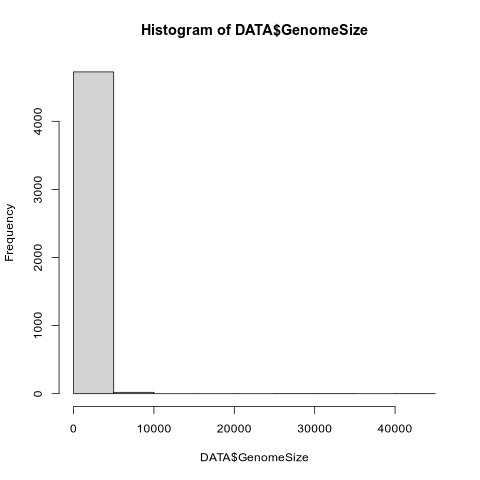
\includegraphics{images/genome_length_animals.png}
\caption{Showing animals genome length distributionbacteria \textless-
read.table(``stats/genomes.bacteria.tbl'', header=FALSE,
comment.char=`\#',
col.names=c(``SpeciesName'',``Superkingdom'',``TaxonGroup'',
``GenomeSize'',``ChromNum''));}
\end{figure}

\hypertarget{further-analyses}{%
\subsection{Further analyses}\label{further-analyses}}

\textbf{IMPORTANT} You can provide here the \texttt{bash} and \texttt{R}
commands to generate the genome sizes histograms for plants, bacteria
(archea not included), and viruses. If you were able to perform and
complete that task, you can play with the data after that and provide
box-plots by taxonomic group showing the distribution of the genome
sizes side-by-side.

\begin{Shaded}
\begin{Highlighting}[]
\CommentTok{\# Your shell commands here}

\CommentTok{\#so we create a .tbl for each case first}

\CommentTok{\# just focus on plant genomes}
\NormalTok{gawk }\StringTok{\textquotesingle{}BEGIN\{ FS=OFS="}\CharTok{\textbackslash{}t}\StringTok{"; \}}
\StringTok{      $2 == "Eukaryota" \&\& $3 == "Plants" \{}
\StringTok{        print $0;}
\StringTok{      \}\textquotesingle{}}\NormalTok{ stats}\OperatorTok{/}\NormalTok{genomes.tbl \textbackslash{}}
       \OperatorTok{\textgreater{}}\StringTok{ }\NormalTok{stats}\OperatorTok{/}\NormalTok{genomes.plants.tbl}

\CommentTok{\# just focus on bacteria genomes}
\NormalTok{gawk }\StringTok{\textquotesingle{}BEGIN\{ FS=OFS="}\CharTok{\textbackslash{}t}\StringTok{"; \}}
\StringTok{      $2 == "Bacteria"\{}
\StringTok{        print $0;}
\StringTok{      \}\textquotesingle{}}\NormalTok{ stats}\OperatorTok{/}\NormalTok{genomes.tbl \textbackslash{}}
       \OperatorTok{\textgreater{}}\StringTok{ }\NormalTok{stats}\OperatorTok{/}\NormalTok{genomes.bacteria.tbl}

\CommentTok{\#Terrabacteria group {-}\textgreater{} Terrabacteria\_group}
\NormalTok{cut }\OperatorTok{{-}}\NormalTok{f3 }\OperatorTok{{-}}\NormalTok{d}\OperatorTok{$}\StringTok{\textquotesingle{}}\CharTok{\textbackslash{}t}\StringTok{\textquotesingle{}}\NormalTok{ stats}\OperatorTok{/}\NormalTok{genomes.bacteria.tbl }\OperatorTok{|}\NormalTok{grep }\StringTok{" "}
\CommentTok{\#find pattern of " "group and unclassified" " among many others, use find and replace to set \_group and unclassified\_}

\CommentTok{\# just focus on virus genomes}
\NormalTok{gawk }\StringTok{\textquotesingle{}BEGIN\{ FS=OFS="}\CharTok{\textbackslash{}t}\StringTok{"; \}}
\StringTok{      $2 == "Viruses"\{}
\StringTok{        print $0;}
\StringTok{      \}\textquotesingle{}}\NormalTok{ stats}\OperatorTok{/}\NormalTok{genomes.tbl \textbackslash{}}
       \OperatorTok{\textgreater{}}\StringTok{ }\NormalTok{stats}\OperatorTok{/}\NormalTok{genomes.virus.tbl}

\NormalTok{cut }\OperatorTok{{-}}\NormalTok{f3 }\OperatorTok{{-}}\NormalTok{d}\OperatorTok{$}\StringTok{\textquotesingle{}}\CharTok{\textbackslash{}t}\StringTok{\textquotesingle{}}\NormalTok{ stats}\OperatorTok{/}\NormalTok{genomes.virus.tbl }\OperatorTok{|}\NormalTok{grep }\StringTok{" "}
\end{Highlighting}
\end{Shaded}

\begin{Shaded}
\begin{Highlighting}[]
\CommentTok{\# Your R commands here}

\NormalTok{animal \textless{}{-}}\StringTok{ }\KeywordTok{read.table}\NormalTok{(}\StringTok{"stats/genomes.animals\_only.tbl"}\NormalTok{,}
                    \DataTypeTok{header=}\OtherTok{FALSE}\NormalTok{, }\DataTypeTok{comment.char=}\StringTok{\textquotesingle{}\#\textquotesingle{}}\NormalTok{,}
                    \DataTypeTok{col.names=}\KeywordTok{c}\NormalTok{(}\StringTok{"SpeciesName"}\NormalTok{,}\StringTok{"Superkingdom"}\NormalTok{,}\StringTok{"TaxonGroup"}\NormalTok{,}
                                \StringTok{"GenomeSize"}\NormalTok{,}\StringTok{"ChromNum"}\NormalTok{));}
\end{Highlighting}
\end{Shaded}

\begin{Shaded}
\begin{Highlighting}[]
\CommentTok{\#first we load the three tables into the R environment}
\NormalTok{plant \textless{}{-}}\StringTok{ }\KeywordTok{read.table}\NormalTok{(}\StringTok{"stats/genomes.plants.tbl"}\NormalTok{,}
                    \DataTypeTok{header=}\OtherTok{FALSE}\NormalTok{, }\DataTypeTok{comment.char=}\StringTok{\textquotesingle{}\#\textquotesingle{}}\NormalTok{,}
                    \DataTypeTok{col.names=}\KeywordTok{c}\NormalTok{(}\StringTok{"SpeciesName"}\NormalTok{,}\StringTok{"Superkingdom"}\NormalTok{,}\StringTok{"TaxonGroup"}\NormalTok{,}
                                \StringTok{"GenomeSize"}\NormalTok{,}\StringTok{"ChromNum"}\NormalTok{));}
\KeywordTok{png}\NormalTok{(}\DataTypeTok{file=}\StringTok{"images/genome\_length\_plants.png"}\NormalTok{, }\DataTypeTok{width=}\DecValTok{800}\NormalTok{, }\DataTypeTok{height=}\DecValTok{600}\NormalTok{, }\DataTypeTok{res=}\DecValTok{150}\NormalTok{);}
\KeywordTok{hist}\NormalTok{(plant}\OperatorTok{$}\NormalTok{GenomeSize);}
\KeywordTok{dev.off}\NormalTok{();}
\end{Highlighting}
\end{Shaded}

\begin{figure}
\centering
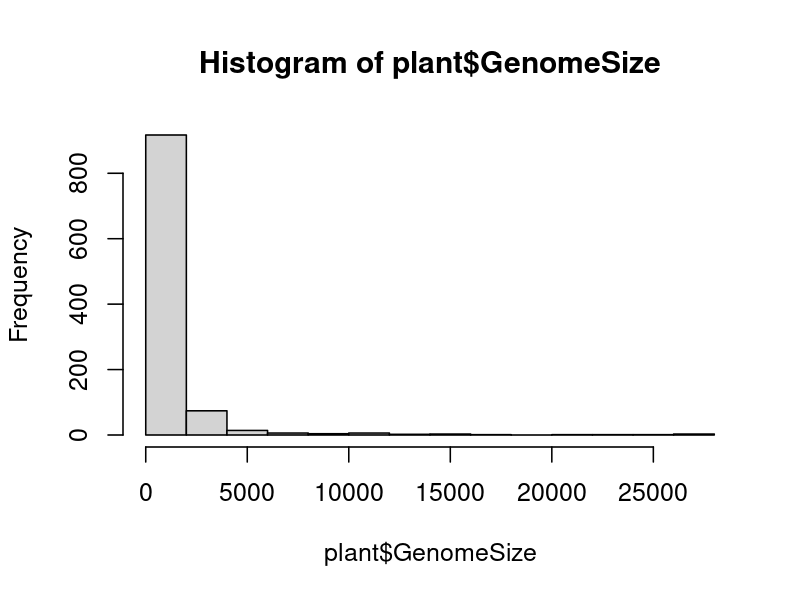
\includegraphics{images/genome_length_plants.png}
\caption{Showing plants genome length distribution}
\end{figure}

\begin{Shaded}
\begin{Highlighting}[]
\NormalTok{bacteria \textless{}{-}}\StringTok{ }\KeywordTok{read.table}\NormalTok{(}\StringTok{"stats/genomes.bacteria.tbl"}\NormalTok{,}
                    \DataTypeTok{header=}\OtherTok{FALSE}\NormalTok{, }\DataTypeTok{comment.char=}\StringTok{\textquotesingle{}\#\textquotesingle{}}\NormalTok{,}
                    \DataTypeTok{col.names=}\KeywordTok{c}\NormalTok{(}\StringTok{"SpeciesName"}\NormalTok{,}\StringTok{"Superkingdom"}\NormalTok{,}\StringTok{"TaxonGroup"}\NormalTok{,}
                                \StringTok{"GenomeSize"}\NormalTok{,}\StringTok{"ChromNum"}\NormalTok{));}

\CommentTok{\#As there were parts that created errors, we used a bash command to fix the data}
\KeywordTok{png}\NormalTok{(}\DataTypeTok{file=}\StringTok{"images/genome\_length\_bacteria.png"}\NormalTok{, }\DataTypeTok{width=}\DecValTok{800}\NormalTok{, }\DataTypeTok{height=}\DecValTok{600}\NormalTok{, }\DataTypeTok{res=}\DecValTok{150}\NormalTok{);}
\KeywordTok{hist}\NormalTok{(bacteria}\OperatorTok{$}\NormalTok{GenomeSize);}
\KeywordTok{dev.off}\NormalTok{();}
\end{Highlighting}
\end{Shaded}

\begin{figure}
\centering
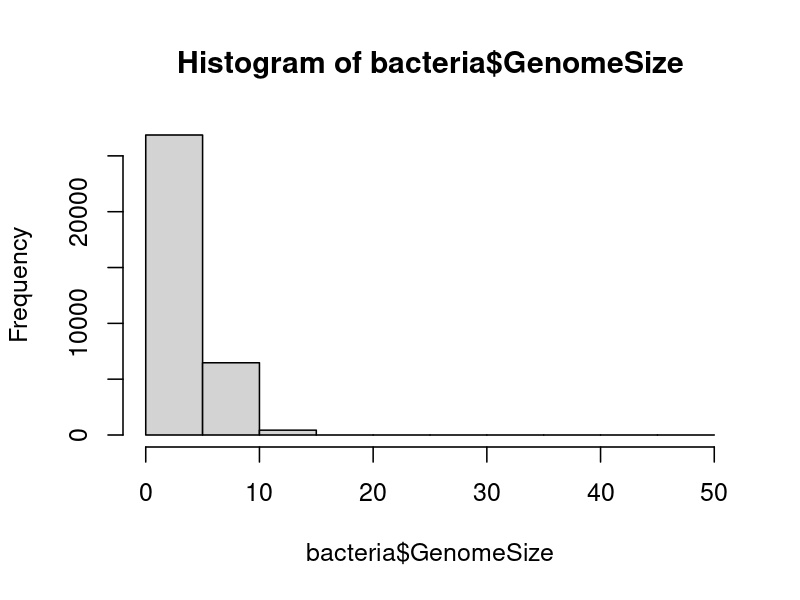
\includegraphics{images/genome_length_bacteria.png}
\caption{Showing plants genome length distribution}
\end{figure}

\begin{Shaded}
\begin{Highlighting}[]
\CommentTok{\#Virus genome plots}
\NormalTok{virus \textless{}{-}}\StringTok{ }\KeywordTok{read.table}\NormalTok{(}\StringTok{"stats/genomes.virus.tbl"}\NormalTok{,}
                    \DataTypeTok{header=}\OtherTok{FALSE}\NormalTok{, }\DataTypeTok{comment.char=}\StringTok{\textquotesingle{}\#\textquotesingle{}}\NormalTok{,}
                    \DataTypeTok{col.names=}\KeywordTok{c}\NormalTok{(}\StringTok{"SpeciesName"}\NormalTok{,}\StringTok{"Superkingdom"}\NormalTok{,}\StringTok{"TaxonGroup"}\NormalTok{,}
                                \StringTok{"GenomeSize"}\NormalTok{,}\StringTok{"ChromNum"}\NormalTok{));}

\CommentTok{\#As there were parts that created errors, we used a bash command to fix the data}
\KeywordTok{png}\NormalTok{(}\DataTypeTok{file=}\StringTok{"images/genome\_length\_virus.png"}\NormalTok{, }\DataTypeTok{width=}\DecValTok{800}\NormalTok{, }\DataTypeTok{height=}\DecValTok{600}\NormalTok{, }\DataTypeTok{res=}\DecValTok{150}\NormalTok{);}
\KeywordTok{hist}\NormalTok{(virus}\OperatorTok{$}\NormalTok{GenomeSize);}
\KeywordTok{dev.off}\NormalTok{();}
\end{Highlighting}
\end{Shaded}

\begin{figure}
\centering
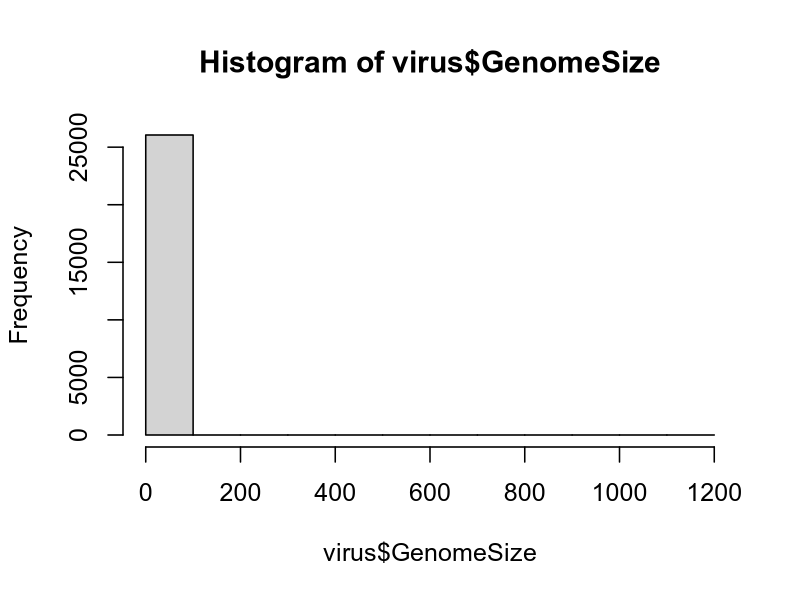
\includegraphics{images/genome_length_virus.png}
\caption{Showing plants genome length distribution}
\end{figure}

\begin{Shaded}
\begin{Highlighting}[]
\CommentTok{\#now the boxplot}
\KeywordTok{library}\NormalTok{(dplyr)}
\KeywordTok{library}\NormalTok{(ggplot2)}
\NormalTok{animal}\OperatorTok{$}\NormalTok{Database\textless{}{-}}\StringTok{"Animals"}
\NormalTok{plant}\OperatorTok{$}\NormalTok{Database\textless{}{-}}\StringTok{"Plants"}
\NormalTok{bacteria}\OperatorTok{$}\NormalTok{Database\textless{}{-}}\StringTok{"Bacteria"}
\NormalTok{virus}\OperatorTok{$}\NormalTok{Database\textless{}{-}}\StringTok{"Virus"}
\NormalTok{data\_joint \textless{}{-}}\StringTok{ }\KeywordTok{bind\_rows}\NormalTok{(animal, plant, bacteria, virus)}
\KeywordTok{ggplot}\NormalTok{(}\DataTypeTok{data=}\NormalTok{data\_joint, }\KeywordTok{aes}\NormalTok{(}\DataTypeTok{x=}\NormalTok{Database, }\DataTypeTok{y=}\NormalTok{GenomeSize, }\DataTypeTok{fill=}\NormalTok{Database))}\OperatorTok{+}
\StringTok{  }\KeywordTok{geom\_boxplot}\NormalTok{()}\OperatorTok{+}\KeywordTok{ggtitle}\NormalTok{(}\StringTok{"Genome sizes across organism groups"}\NormalTok{)}\OperatorTok{+}\KeywordTok{theme}\NormalTok{(}\DataTypeTok{plot.title =} \KeywordTok{element\_text}\NormalTok{(}\DataTypeTok{hjust =} \FloatTok{0.5}\NormalTok{))}
\KeywordTok{ggsave}\NormalTok{(}\DataTypeTok{file=}\StringTok{"images/genome\_boxplot\_comparison.png"}\NormalTok{, }\DataTypeTok{width =} \DecValTok{9}\NormalTok{, }\DataTypeTok{height =} \DecValTok{7}\NormalTok{)}
\end{Highlighting}
\end{Shaded}

\begin{figure}
\centering
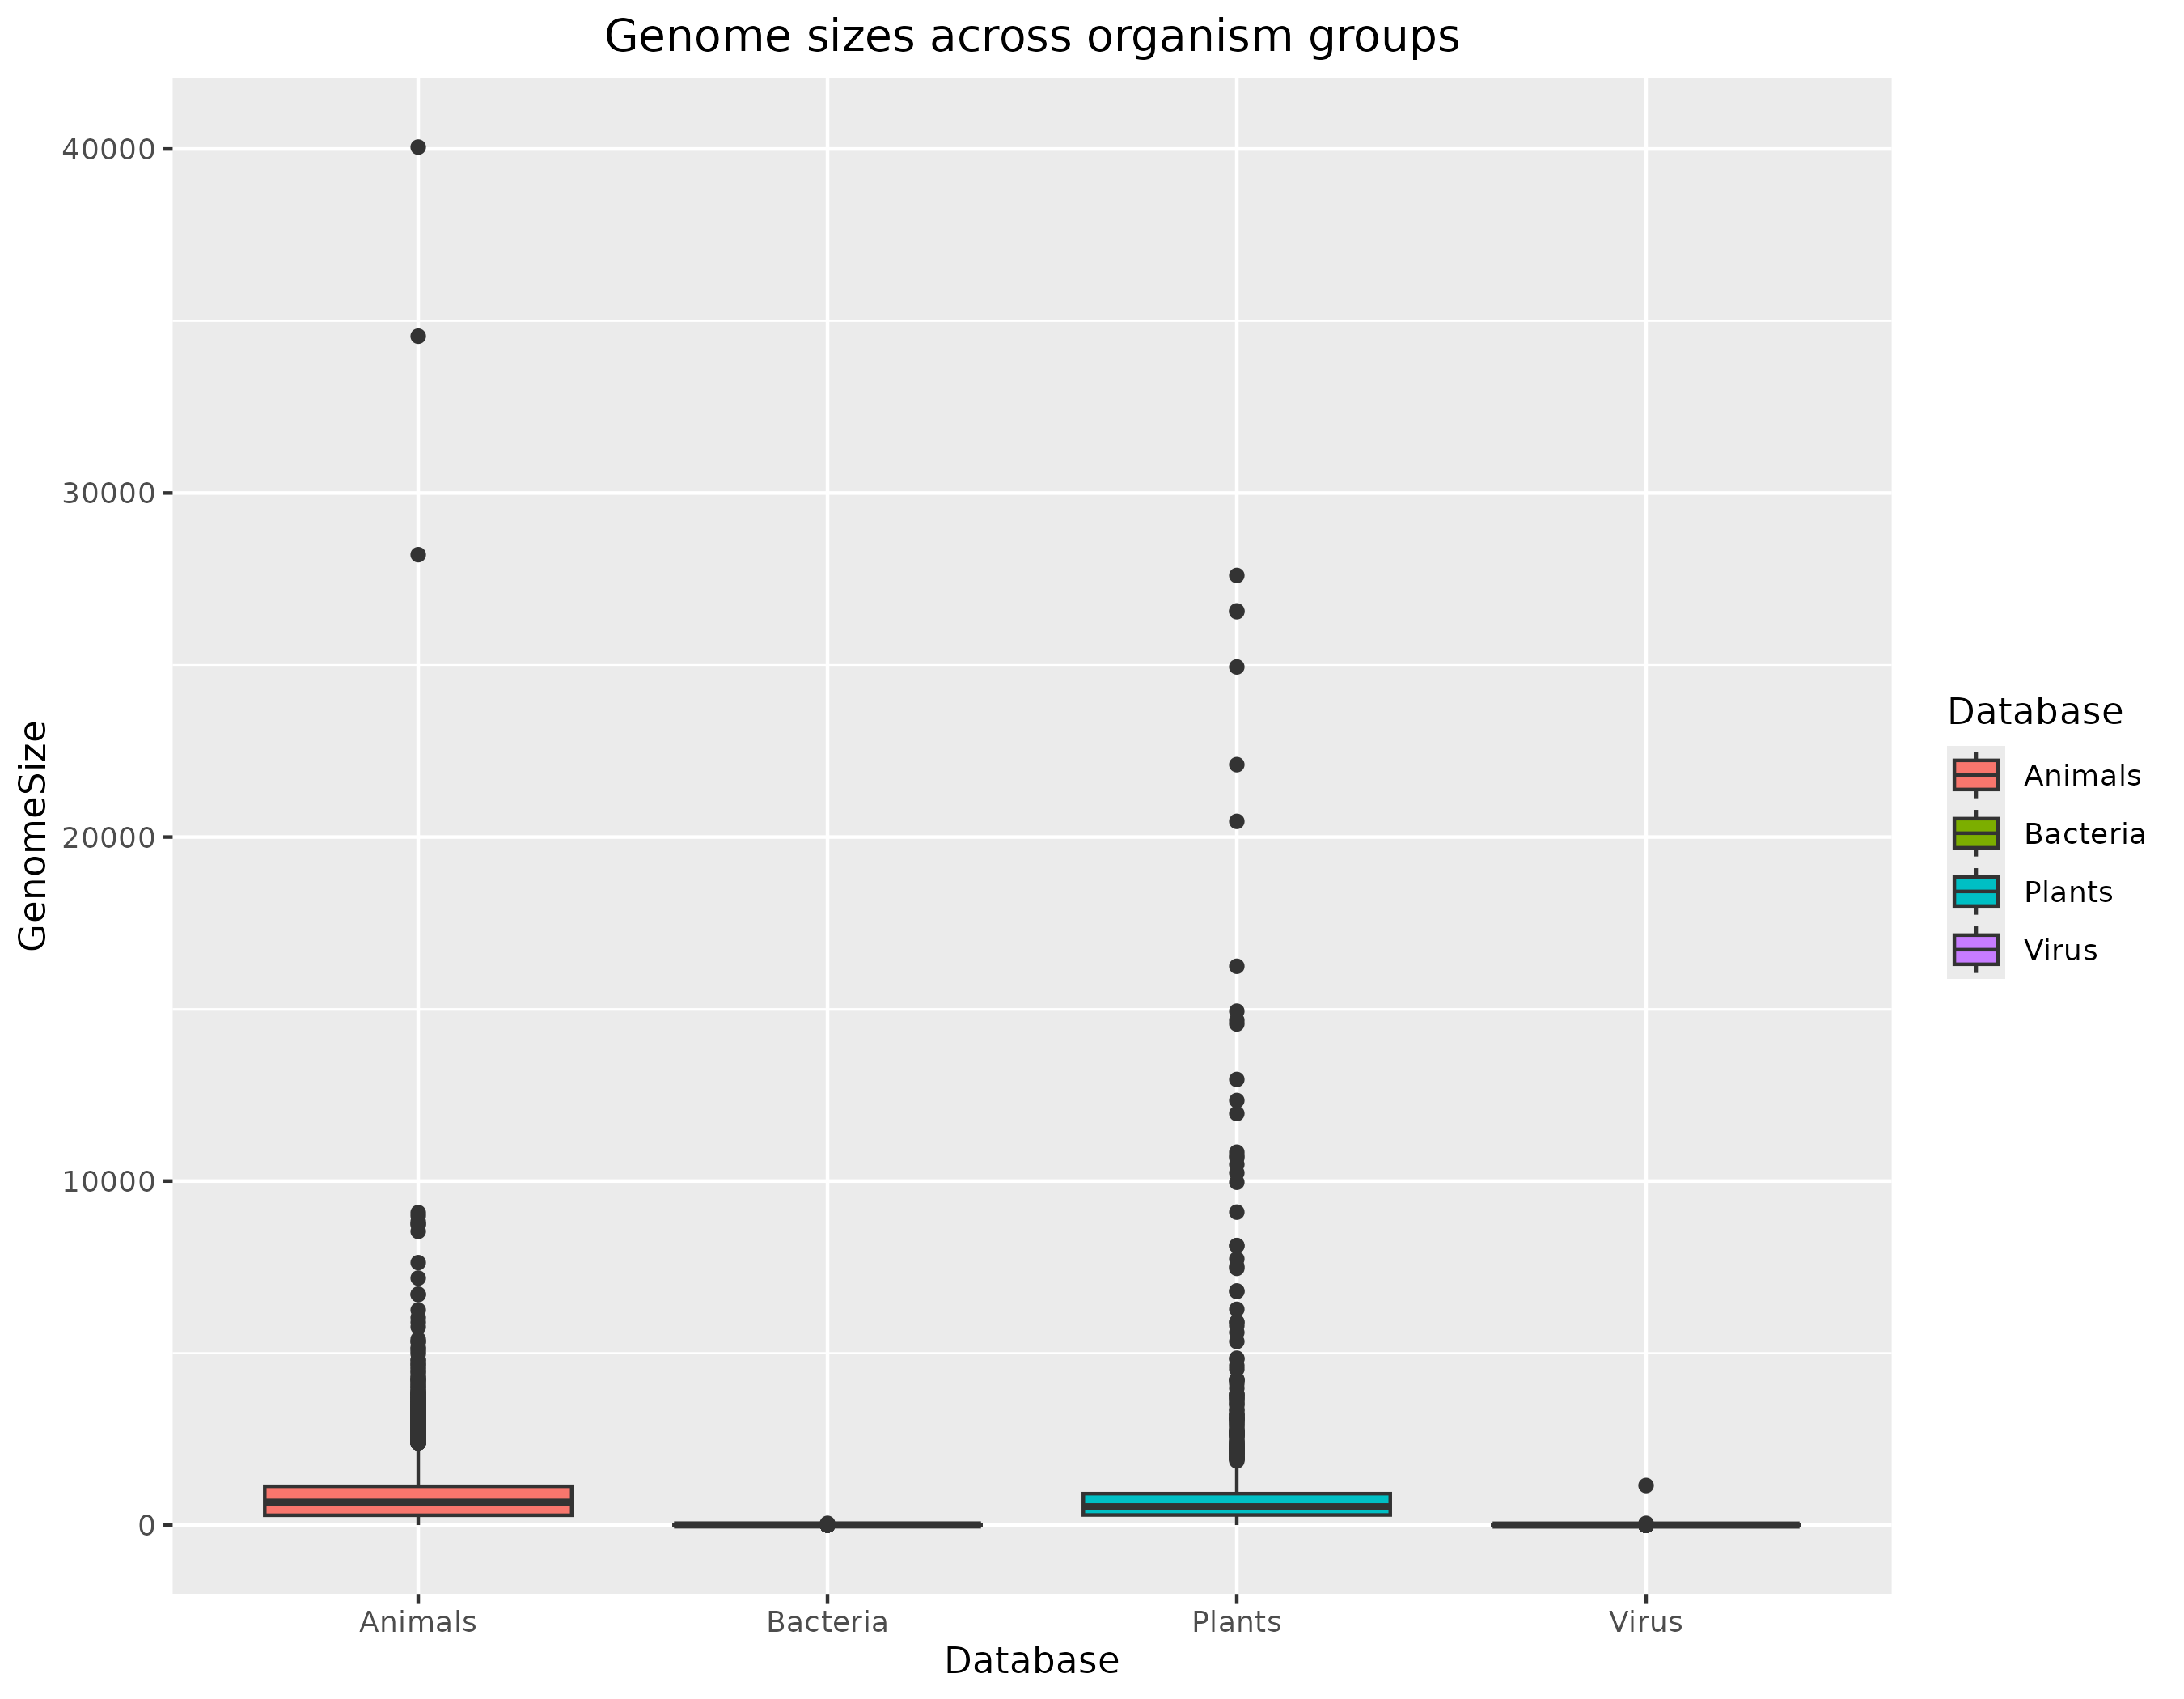
\includegraphics{images/genome_boxplot_comparison.png}
\caption{Showing plants genome length distribution}
\end{figure}

\hypertarget{discussion}{%
\section{Discussion}\label{discussion}}

\label{sec:discussion}

\textbf{IMPORTANT} Discuss your results here (around 300 words). And
remember to include in the Appendices section (see page
\pageref{sec:appendices}), any extra script you wrote from this exercise
\texttt{bin} folder using the \texttt{loadfile} macro.

:: All of the organism groups have a high frequency of small genome
sizes, as can be seen from the histograms of each individual group. We
can also see in the box plots that the genome sizes of eukaryotes, or
plants and animals, are larger than those of bacteria and viruses. It is
also evident that, of all the groups, plants have the highest frequency
of large genomes; nevertheless, animals have the largest genome sizes.
::

\clearpage

\hypertarget{appendices}{%
\section{Appendices}\label{appendices}}

\label{sec:appendices}

\hypertarget{software}{%
\subsection{Software}\label{software}}

We have used the following versions:

\begin{Shaded}
\begin{Highlighting}[]
\FunctionTok{uname}\NormalTok{ {-}a}
\CommentTok{\# Linux aleph 5.15.0{-}117{-}generic \#127{-}Ubuntu SMP}
\CommentTok{\# Fri Jul 5 20:13:28 UTC 2024 x86\_64 x86\_64 x86\_64 GNU/Linux}

\ExtensionTok{R}\NormalTok{ {-}{-}version}
\CommentTok{\# R version 4.3.1 (2023{-}06{-}16) {-}{-} "Beagle Scouts"}
\CommentTok{\# Copyright (C) 2023 The R Foundation for Statistical Computing}
\CommentTok{\# Platform: x86\_64{-}conda{-}linux{-}gnu (64{-}bit)}

\FunctionTok{wget}\NormalTok{ {-}{-}version}
\CommentTok{\# GNU Wget 1.21.2 built on linux{-}gnu.}

\ExtensionTok{pandoc}\NormalTok{ {-}{-}version}
\CommentTok{\# pandoc 3.1.3}
\CommentTok{\# Features: +server +lua}
\CommentTok{\# Scripting engine: Lua 5.4}

\ExtensionTok{mamba}\NormalTok{ {-}{-}version}
\CommentTok{\# mamba 1.4.2}
\CommentTok{\# conda 23.3.1}
\end{Highlighting}
\end{Shaded}

\hypertarget{supplementary-files}{%
\subsection{Supplementary files}\label{supplementary-files}}

\label{sec:supplfiles}

\hypertarget{conda-environment-dependencies-for-the-exercise}{%
\subsubsection{\texorpdfstring{\texttt{conda} environment dependencies
for the
exercise}{conda environment dependencies for the exercise}}\label{conda-environment-dependencies-for-the-exercise}}

\loadfile{environment.yml}{environment.yml}{prg:environmentYML}

\hypertarget{project-specific-scripts}{%
\subsubsection{Project specific
scripts}\label{project-specific-scripts}}

\loadfile{an\_script\_example.pl}{bin/an_script_example.pl}{prg:scriptexamplePERL}

\hypertarget{shell-global-vars-and-settings-for-this-project}{%
\subsubsection{Shell global vars and settings for this
project}\label{shell-global-vars-and-settings-for-this-project}}

\loadfile{projectvars.sh}{projectvars.sh}{prg:projectvarsBASH}

\hypertarget{about-this-document}{%
\subsection{About this document}\label{about-this-document}}

This document was be compiled into a PDF using \texttt{pandoc} (see
\texttt{projectvars.sh} from previous subsection) and some
\texttt{LaTeX} packages installed in this linux system.
\texttt{synaptic}, \texttt{apt-get} or \texttt{aptitude} can be used to
retrieve and install those tools from linux repositories. As the
\texttt{raw\_tex} extension has been provided to the
\texttt{markdown\_github} and \texttt{tex\_math\_dollars} formats, now
this document supports inline \LaTeX~and inline formulas!

You can get further information from the following links about the
\href{http://daringfireball.net/projects/markdown/syntax\#link}{Mark
Down syntax}, as well as from the manual pages (just type
\texttt{man\ pandoc} and/or \texttt{man\ pandoc\_markdown}).


\end{document}
